\documentclass[xcolor=dvipsnames,8pt,handout]{beamer}
%\documentclass[xcolor=dvipsnames,8pt]{beamer}
\usepackage{multirow}
\usepackage{scrextend}
\usepackage[square,super]{natbib} %citep and citet
\usetheme{Sybila}
\linespread{1.4} %调整行间距
\graphicspath{{figure/}}
\usepackage[export]{adjustbox}
\title[结构设计原理]{极限状态设计法的可靠指标与实用设计表达式之间的
  关系}
\author[哈尔滨工业大学交通科学与工程学院]{\songti 杨大伟 \quad  吕大刚 }
\date{2016.8.23-25, 长沙\\ 第二届全国《结构设计原理》课程教学研讨会}
% 符合表
\newcommand{\var}[2]{#1_\mathrm{#2}}
\newcommand{\Mdu}{M_{\mathrm{du}}}
\newcommand{\MGK}{M_{\mathrm{GK}}}
\newcommand{\Md}{M_{\mathrm{d}}}
\newcommand{\Ac}{A_\mathrm{c}}
\newcommand{\Ec}{E_\mathrm{c}}
\newcommand{\Es}{E_\mathrm{s}}
\newcommand{\Gc}{G_\mathrm{c}}
\newcommand{\Asb}{A_\mathrm{sb}}
\newcommand{\Asv}{A_\mathrm{sv}}
\newcommand{\As}{A_\mathrm{s}}
\newcommand{\Vd}{V_\mathrm{d}}
\newcommand{\Sv}{S_\mathrm{v}}
\newcommand{\Qd}{Q_\mathrm{d}}
\newcommand{\fcd}{f_\mathrm{cd}}
\newcommand{\fcc}{f_\mathrm{cc}}
\newcommand{\fc}{f_\mathrm{c}}
\newcommand{\fk}{f_\mathrm{k}}
\newcommand{\ak}{a_\mathrm{k}}
\newcommand{\pf}{P_\mathrm{f}}
\newcommand{\ps}{P_\mathrm{s}}
\newcommand{\pfk}{P_\mathrm{fk}}
\newcommand{\ur}{\sigma_\mathrm{r}}
\newcommand{\fcuk}{f_\mathrm{cu,k}}
\newcommand{\fsdv}{f_\mathrm{sd,v}}
\newcommand{\fsdb}{f_\mathrm{sd,b}}
\newcommand{\fsd}{f_\mathrm{sd}}
\newcommand{\fck}{f_\mathrm{ck}}
\newcommand{\ftk}{f_\mathrm{tk}}
\newcommand{\ho}{h_\mathrm{0}}
\newcommand{\xb}{x_\mathrm{b}}
\newcommand{\xib}{\xi_\mathrm{b}}
\newcommand{\yc}{y_\mathrm{c}}
\newcommand{\gammas}[1]{\gamma_\mathrm{#1}}
\newcommand{\Ss}[1]{S_\mathrm{#1}}

\newcommand{\sigmas}{\sigma_\mathrm{s}}
\newcommand{\sigmac}{\sigma_\mathrm{c}}
\newcommand{\sigmao}{\sigma_\mathrm{0}}
\newcommand{\sigmaM}{\sigma_\mathrm{M}}
\newcommand{\sigmaR}{\sigma_\mathrm{R}^2}
\newcommand{\sigmaS}{\sigma_\mathrm{S}^2}
\newcommand{\vac}{\varepsilon_\mathrm{c}}
\newcommand{\vao}{\varepsilon_\mathrm{o}}
\newcommand{\vacu}{\varepsilon_\mathrm{cu}}




\newcommand{\kn}{\ \mathrm{kN\cdot m}}
\newcommand{\mm}{\ \mathrm{mm}}
\newcommand{\mpa}{\ \mathrm{MPa}}
\newcommand{\ufcs}{\mu_\mathrm{{fc}}^{s}}
\newcommand{\ufs}{\mu_\mathrm{{f150}}^{s}}
\newcommand{\ufc}{\mu_\mathrm{fc}}
\newcommand{\uo}{\mu_\mathrm{\Omega 0}}
\newcommand{\uM}{\mu_\mathrm{M}}
\newcommand{\uR}{\mu_\mathrm{R}}
\newcommand{\uS}{\mu_\mathrm{S}}
\newcommand{\fvs}{f_\mathrm{{\nu}}^{s}}
\newcommand{\fcs}{f_\mathrm{c}^{s}}
\newcommand{\fts}{f_\mathrm{t}^{s}}
\newcommand{\fcus}{f_\mathrm{cu}^{s}}



\renewcommand{\vec}[2]{\mathbf{#1}_\mathrm{#2}}
\newcommand{\tranvec}[2]{\mathbf{#1}$^{\mathrm{'}}$ $_{\mathrm{#2}}$}
\newcommand{\lqg}[4]{\tranvec{#1}{#2}(#4)\mathbf{#3}(#4)\vec{#1}{#2}(#4)}
\providecommand{\alert}[1]{\textbf{#1}}

\newcommand{\ut}{\mathbf{T}}
\newcommand{\uti}[1]{\mathbf{T}^{(#1)}}
\newcommand{\uts}{\mathbf{T}^{*}}
\newcommand{\iut}[1]{\mathbf{T}_{#1}}

\newcommand{\lt}{\mathbf{t}}
\newcommand{\lti}[1]{\mathbf{t}^{(#1)}}
\newcommand{\lts}{\mathbf{t}^{*}}
\newcommand{\ilt}[1]{\mathbf{t}_{#1}}
\newcommand{\pt}{\dfrac{\partial \ut}{\partial \lt}}
\newcommand{\dut}{\Delta \mathbf{T}}
\newcommand{\duti}[1]{\Delta \mathbf{T}^{(#1)}}
\newcommand{\dTdt}{\dfrac{\partial \ut}{\partial \lt}}
\newcommand{\dSdt}{\dfrac{\partial \us}{\partial \lt}}
\newcommand{\ltsi}[1]{\mathbf{t}^{*(#1)}}
\newcommand{\us}{\mathbf{S}}
\newcommand{\usi}[1]{\mathbf{S}^{(#1)}}
\newcommand{\uss}{\mathbf{S^*}}
\newcommand{\ussi}[1]{\mathbf{S^*}^{(#1)}}

\newcommand{\alphai}[1]{\mathbf{\alpha}^{(#1)}} 
\newcommand{\alphaij}[2]{\mathbf{\alpha}_{#2}^{(#1)}}
\newcommand{\alphao}{\mathbf{\alpha_{\rm{I}}}}
\newcommand{\alphal}{\mathbf{\alpha_{\rm{II}}}}
\newcommand{\dTdti}[1]{\dfrac{\partial \uti{#1}}{\partial \lt^{(#1)}}}
\newcommand{\dSdti}[1]{\dfrac{\partial \usi{#1}}{\partial \lti{#1}}}
\newcommand{\ug}{\mathbf{G}}
\newcommand{\dTdtik}[1]{\dfrac{\partial \mathbf{T}^{(i)}}{\partial t^{(i)}_{#1}}}     
\newcommand{\floor}[1]{\lfloor{#1}\rfloor}
\newcommand{\before}[2]{{#1}{\rightarrowtail}{#2}}
\newcommand{\after}[2]{{#1}{\leftarrowtail}{#2}}
\newcommand{\together}[2]{{#1}{\leftrightarrows}{#2}}
% \newcommand{\lts}{\mathbf{t}^{*}}

\newcommand\Tx{\vec{T}{x}}
\newcommand\Tu{\vec{T}{u}}
\newcommand\Tk{\mathbf{T}(k)}

\newcommand\xk{\mathbf{x}(k)}
\newcommand\xko{\mathbf{x}(k_0)}
\newcommand\xkf{\mathbf{x}(k_f)}
\newcommand\uk{\mathbf{u}(k)}
\newcommand\zk{\mathbf{z}(k)}
\newcommand\zkf{\mathbf{z}(k_f)}
\newcommand\yk{\mathbf{y}(k)}
\newcommand\ek{\mathbf{e}(k)}        
\newcommand\Pk{\mathbf{P}(k)}
\newcommand\Pkk{\mathbf{P}(k+1)}
\newcommand\Pkf{\mathbf{P}(k_f)}
\newcommand\gk{\mathbf{g}(k)}
\newcommand\gkk{\mathbf{g}(k)}
\newcommand\gkf{\mathbf{g}(k_f)}
\newcommand\Lk{\mathbf{L}(k)}
\newcommand\Lg{\mathbf{L_g}(k)}
\newcommand\Lgk{\mathbf{L_g}(k)}
\newcommand\xsk{\mathbf{x^*}(k)}
\newcommand\xskk{\mathbf{x^*}(k+1)}
\newcommand\usk{\mathbf{u^*}(k)}

%%% Local Variables:
%%% mode: plain-tex
%%% TeX-master: "../main"
%%% End:
  %定义数学符号

\begin{document}

\begin{frame}[plain]
   \titlepage 
\end{frame}

\begin{frame}[t]
  \frametitle{前言}
  \begin{itemize}
  \item<1-> \textbf{概念回顾}
    \begin{itemize}
    \item 结构设计中的不确定性
    \item 极限状态与极限状态方程
    \item 承载能力极限状态和正常使用极限状态
    \item 实用设计表达式
    \end{itemize}
  \item<2-> \textbf{疑问}
    \begin{itemize}
    \item<3-> 为什么设计方法\underline{以概率理论为基础}或在设计中设定
      了目标可靠指标$\var{\beta}{T}$,工程师却没有
      在设计实践中计算\underline{结构可靠度}或\underline{失效概率}?
      \begin{equation}
      \label{probabiliy}
      %\ps = P(g(r,s)>0)  = \iint_{g>0} \var{f}{R}(r) \var{f}{S}(s)
      %  \mathrm{d}r\mathrm{d}s \\ \nonumber
      \pf = \iint_{g(r,s)<0} \var{f}{R}(r)
        \var{f}{S}(s)\mathrm{d}r\mathrm{d}s 
      \end{equation}
或
      \begin{equation}
     \pf = \idotsint_{g(\mathbf{X})<0}
        \var{f}{x_{1}}(x_{1})\var{f}{x_{2}}(x_{2})\cdots\var{f}{x_{n}}(\var{x}{n})
        \mathrm{d}{x_{1}} \mathrm{d}{x_{2}}\cdots
        \mathrm{d}{\var{x}{n}}
      \end{equation}

    \item<4-> 实用设计表达式与\underline{可靠度}之间有什么样的关系?设
      计值或分项系数是如何被确定的?(式\eqref{eq:limit}为作用效应基本
      组合的极限状态设计表达式,以下均以此式为讨论对象。)
      \begin{equation}
      \label{eq:limit}
      \textcolor{red}{\gammas{0}}(\sum_{i=1}^{{m}}\textcolor{red}{\gammas{Gi}}\Ss{Gik}+\textcolor{red}{\gammas{Q1k}}\Ss{Q1k}+\textcolor{red}{\Psi_{\mathrm{c}}}\sum_{j=2}^{n}\textcolor{red}{\gammas{Qj}}\Ss{Qjk})
      \leqslant \textcolor{red}{\dfrac{1}{\gammas{R}}}R(\textcolor{red}{\gammas{f}},\fk,\ak)
      \end{equation}
    \end{itemize}
   \end{itemize}
\end{frame}

\begin{frame}[t]
  \frametitle{教学目标和内容 }
   \onslide<1->
    \begin{note}
      \underline{可靠指标}与\underline{实用设计表达式}之间的联系即
      \emph{分项安全系数},简称\underline{分项系数}。
    \end{note}
  \begin{itemize}
    \item<2-> \textbf{目标}
    \begin{itemize}
    \item<2-> 解释可靠指标与分项系数之间的关系;
    \item<2-> 了解实用设计表达式中的分项系数是如何确定的。
    \end{itemize}
    \item<3-> \textbf{内容}
    \begin{itemize}
    \item<3-> 分项系数的推导;
    \item<3-> 分项系数和可靠指标的几何解释;
    \item<3-> 确定分项系数的方法。
    \end{itemize}
  \end{itemize}
\end{frame}

\begin{frame}[t]
  \frametitle{可靠度及可靠指标}
    \begin{labeling}{可靠度指标}
      \item<1-> [\textbf{可靠度}\cite{D62-2004,Gong2007}] 结构在规定的时间内,
        在规定的条件下,完成预定功能的概率。它是结构可靠性的概率度量,
        用$\var{P}{s}$表示。
      \item<2-> [\textbf{失效概率}] 一般使用失效概率描述结构的可靠度:
        $\var{P}{f}=1-\var{P}{s}$。
        \begin{center}
          \onslide<3->{$\var{P}{f}=2.3 \times 10^{-4}$
            vs. $\var{P}{s}=0.999977$}
        \end{center}
      \item<4-> [\textbf{可靠指标}] 与\underline{失效概率}对应的指标。当功能函数
        $g$服从正态分布即$g \sim N(\var{\mu}{g},\var{\sigma}{g}^{2})$时:
        \begin{center}
          \onslide<5->{$\var{P}{f}=\Phi(-\beta)$,其中
          $\beta=\dfrac{\var{\mu}{g}}{\var{\sigma}{g}}$}
        \end{center}
        \onslide<6->{当$g$不服从正态分布时,采用近似计算方法(FORM)计算$\beta$。}
    \end{labeling}

    \begin{figure}[H]
      \centering
      \includegraphics<7->[height=3cm]{beta.png}
      \onslide<7->{\caption{极限状态$g(\cdot)$概率密度\cite{Choi2007}}}
    \end{figure}
\end{frame}

\begin{frame}[t]
  \frametitle{功能函数的可靠指标\cite{GB50283-1999}}
  \begin{itemize}
  \item \textbf{定义}:假定$R\sim N(\var{\mu}{R},\var{\sigma}{R}^{2})$,$S\sim
    N(\var{\mu}{S},\var{\sigma}{S}^{2})$且相互独立,

  \begin{equation}
    \label{fun}
    g(R,S) = R - S
  \end{equation}
  
  \item \textbf{推导}:
 
  由$\var{\mu}{g} = \var{\mu}{R}- \var{\mu}{S}$,$ \var{\sigma}{g} =
  \sqrt{ \var{\sigma}{R}^{2} + \var{\sigma}{S}^{2}}$得:

  \begin{equation}
    \label{beta}
    \beta = \dfrac{\var{\mu}{R}- \var{\mu}{S}}{\sqrt{\var{\sigma}{R}^{2}+ \var{\sigma}{S}^{2}}}
  \end{equation}

  %当计算得到可靠度指标$\beta$后,即计算得到失效概率:
  %\begin{equation}
  %  \pf = \Phi({\dfrac{0-\mu_{g}}{\sigma_{g}}})= \Phi(-\beta)
  %\end{equation}
  \item \textbf{功能函数转换至标准空间}
    
  将$\var{R}{u}=(R-\var{\mu}{R})/\var{\sigma}{R}$和
  $\var{S}{u}=(S-\var{\mu}{S})/\var{\sigma}{S}$代入\eqref{fun}得:
  \begin{equation}
  \label{eq:standard}
    g(\var{R}{u},\var{S}{u}) = \var{R}{u}\var{\sigma}{R} + \var{\mu}{R} -
    \var{S}{u}\var{\sigma}{S} - \var{\mu}{S} = 0
  \end{equation}
  \end{itemize}
\end{frame}

\begin{frame}
  \frametitle{原始空间与标准空间(X to U)}
  \begin{figure}[H]
    \centering
    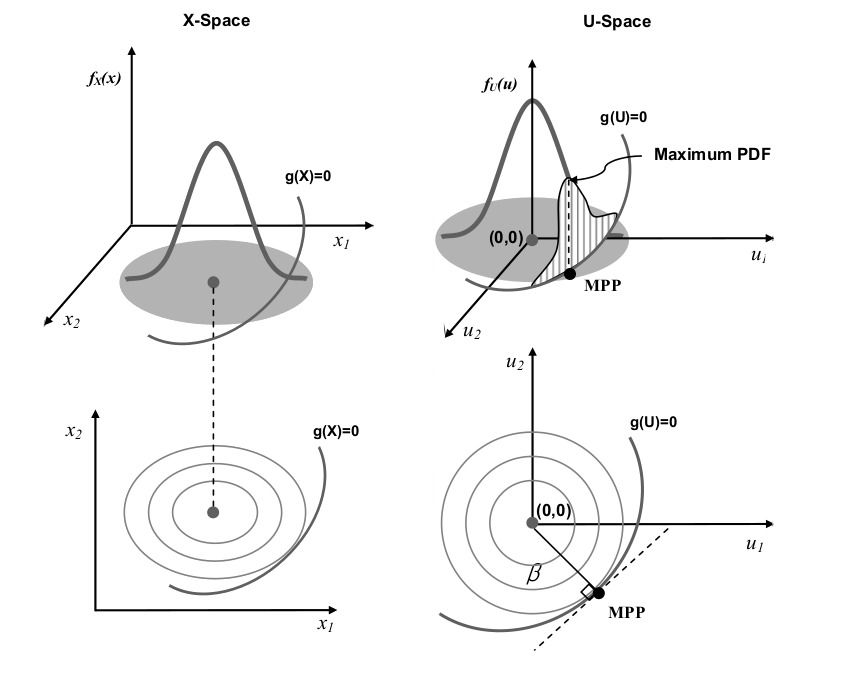
\includegraphics[height=0.7\textheight]{trans.png} 
    \caption{随机变量空间转换\cite{Choi2007}}
  \end{figure}
\end{frame}

\begin{frame}[t]
  \frametitle{设计点求解}
  \begin{columns}[t]
  \begin{column}{0.6\textwidth}
    
  \onslide<2->{%
  对式\eqref{eq:standard}作变换,方程两边同除以
  $- \sqrt{\var{\sigma}{R}^{2}+\var{\sigma}{S}^{2}}$得:
  \begin{equation}
    \label{eq:trans}
    - \dfrac{\var{\sigma}{R}}{\sqrt{\var{\sigma}{R}^{2}+\var{\sigma}{S}^{2}}}\var{R}{u} +
    \dfrac{\var{\sigma}{S}}{\sqrt{\var{\sigma}{R}^{2}+\var{\sigma}{S}^{2}}}\var{S}{u}
    -
    \dfrac{\var{\mu}{R}-\var{\mu}{S}}{\sqrt{\var{\sigma}{R}^{2}+\var{\sigma}{S}^{2}}}=0
  \end{equation}
  }%

  \onslide<3->{%
  求解标准空间中原点距该直线的距离$\beta$及垂足坐标:
  \begin{eqnarray}
    \label{eq:beta}
    \beta =
    \dfrac{\var{\mu}{R}-\var{\mu}{S}}{\sqrt{\var{\sigma}{R}^{2}+\var{\sigma}{S}^{2}}} \\
    \var{R}{ud} = \cos{\theta_{R_{
\mathrm{ud}}}} \beta = - \dfrac{\var{\sigma}{R}}{\sqrt{\var{\sigma}{R}^{2}+\var{\sigma}{S}^{2}}}\beta \\
    \var{S}{ud} = \cos{\theta_{S_{
\mathrm{ud}}}} \beta = \dfrac{\var{\sigma}{S}}{\sqrt{\var{\sigma}{R}^{2}+\var{\sigma}{S}^{2}}}\beta
  \end{eqnarray}
  }%
  \end{column}
  \begin{column}{0.4\textwidth}
    \begin{figure}[t]
     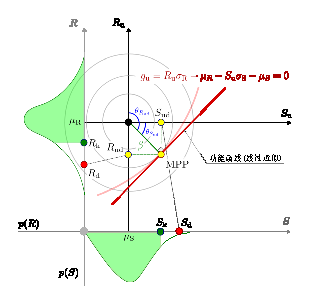
\includegraphics[width=\textwidth]{normalspace.eps} 
    \end{figure}
  \end{column}
  \end{columns}
  \onslide<4->{%
该垂足点即为\underline{最可能失效点},也就是\underline{设计值点},变换至原空间得:
  \begin{equation}
    \label{eq:transs}
    \var{R}{d} = \var{\mu}{R} + \var{R}{ud}\var{\sigma}{R} \quad
    \var{S}{d} = \var{\mu}{S} + \var{S}{ud}\var{\sigma}{S}
  \end{equation}
  }%
\end{frame}

\begin{frame}[t]
  \frametitle{分项安全系数}
  \begin{columns}[t]
  \begin{column}{0.6\textwidth}
    \onslide<2->{%
  定义:$\var{\alpha}{R} = -\cos(\var{\theta}{R_{ud}})$和
  $\var{\alpha}{S} = \cos(\var{\theta}{S_{ud}})$
  代入式\eqref{eq:transs}得\underline{设计点表达式}:
  \begin{eqnarray}
    \var{R}{d} = \var{\mu}{R} - \var{\alpha}{R}\beta\var{\sigma}{R} =
    \var{\mu}{R}(1 - \var{\alpha}{R}\beta\var{\delta}{R}) \\
    \var{S}{d} = \var{\mu}{S} + \var{\alpha}{S}\beta\var{\sigma}{S} =
    \var{\mu}{S}(1 + \var{\alpha}{S}\beta\var{\delta}{S}) 
  \end{eqnarray}
  }%
  \onslide<3->{%
  定义抗力和荷载效应的\underline{标准值}分别为$\var{R}{k}$和
  $\var{S}{k}$:
  \begin{eqnarray}
    \var{R}{k} = \var{\mu}{R}(1-\var{\theta}{R}\var{\delta}{R}) \\
    \var{S}{k} = \var{\mu}{S}(1+\var{\theta}{S}\var{\delta}{S})
  \end{eqnarray}
   }%
  \end{column}
  \begin{column}{0.4\textwidth}
    \begin{figure}[t]
     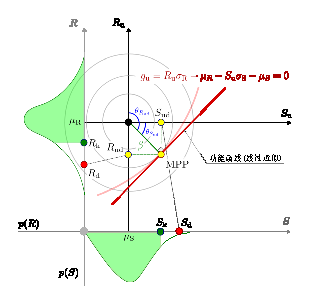
\includegraphics[width=\textwidth]{normalspace.eps} 
    \end{figure}
  \end{column}
  \end{columns}
  \onslide<4->{%}
  则(非严格)定义分项安全系数:
  \begin{eqnarray}
    \dfrac{1}{\var{\gamma}{R}} = \dfrac{\var{R}{d}}{\var{R}{k}} =
    \dfrac{\var{\mu}{R}(1-\var{\alpha}{R}\beta\var{\delta}{R})}{\var{\mu}{R}(1-1.645\var{\delta}{R})}
    = \dfrac{1-\var{\alpha}{R}\textcolor{red}{\beta}\var{\delta}{R}}{1-\var{\theta}{R}\var{\delta}{R}}\\
    \var{\gamma}{S} = \dfrac{\var{S}{d}}{\var{S}{k}} =
    \dfrac{\var{\mu}{S}(1+\var{\alpha}{S}\beta\var{\delta}{S})}{\var{\mu}{S}(1+1.645\var{\delta}{S})}
    = \dfrac{1+\var{\alpha}{S}\textcolor{red}{\beta}\var{\delta}{S}}{1+\var{\theta}{S}\var{\delta}{S}}
  \end{eqnarray}
  }%
  \onslide<5->{%}
 \small
  \textbf{注}:{\kaishu 式中$\var{\gamma}{R}$对应实用表达式\eqref{eq:limit}中的
  $\var{\gamma}{f}$,意指材料强度分项系数。式\eqref{eq:limit}中的
  $\var{\gamma}{R}$为结构抗力计算模式不定性系数。}
  }%
\end{frame}

\begin{frame}
  \frametitle{分项系数几何解释}
  \begin{figure}[H]
    \centering
    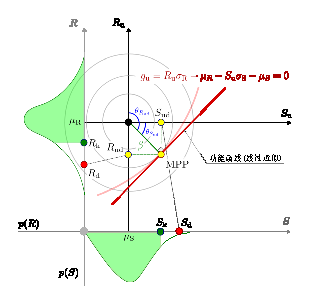
\includegraphics[height=0.8\textheight]{normalspace.eps}
  \end{figure}
\end{frame}

\begin{frame}
  \frametitle{重要性系数}
  \begin{discuss}
  由于实际工程中结构可靠性还和\underline{结构的安全等级}有关,为了便
  于适应不同安全等级的可靠指标$\var{\beta}{T}$,在实用设计表达式中引
  入了\underline{结构重要性系数$\var{\gamma}{0}$}。
  这样在参量设计值保持不变的前提下,仅通过调整$\var{\gamma}{0}$即可使
  结构设计获得不同的可靠度。  
    \end{discuss}
\end{frame}

\begin{frame}
  \frametitle{重要性系数}
    \begin{figure}[H]
      \centering
      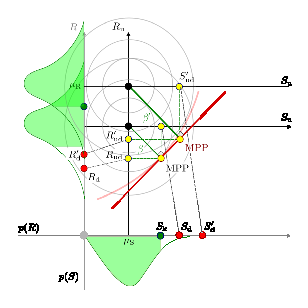
\includegraphics[height=0.8\textheight]{betamore.eps}
    \end{figure}
\end{frame}

\begin{frame}[t]
  \frametitle{分项安全系数}
       \begin{itemize}
       \item<2-> 分项安全系数(partial safety factors)表征的是与特定
         目标可靠度对应的\underline{设计值}与\underline{标准值}间的\underline{关系}。
         \item<3-> \underline{设计值}源于最可失效点的求解,其几何意义为标准空间原点到
           极限状态曲线的垂足。 
         \item<4-> \underline{标准值}是参数的代表值或特征值,它是参数
           在某种特征意义上的定义值。
         \item<5-> 参数的随机特征是\underline{客观既定的},目标可靠度
           $\var{\beta}{T}$却是\underline{主观决定的}。
       \end{itemize} 
  
  \onslide<6->{%
  \begin{note}
   1. 将\underline{可靠度设计}转化为\underline{基于设计值的极限状态方程求解},从而避免了复杂的
   可靠度分析。

   2. 可通过调整可靠度指标$\var{\beta}{T}$,改变结构可靠度;而$\var{\beta}{T}$的改变也导致了设计值的改变。
   \end{note}
  }%
\end{frame}

\begin{frame}[t]
  \frametitle{设计值方法}
  \onslide<1->{%
  \textbf{已知}:
  \begin{enumerate}
  \item 设计参量$\var{x}{i}$、其所服从的随机分布$\var{F}{X_{i}}$;
  \item 功能函数$g(\var{X}{1},\var{X}{2},\cdots,\var{X}{n})$; 
  \item 目标可靠度$\var{\beta}{T}$。
  \end{enumerate}
  }%
  \onslide<2->{%
  \textbf{求}:结构实用设计表达式中的设计值或分项系数
  \begin{equation}
    g(\var{x}{1d},\var{x}{2d},\cdots,\var{x}{nd}) \geqslant 0 \quad 
    \text{或} \quad
    g(\var{\gamma}{X_{1}}{\var{x}{1k}},\var{\gamma}{X_{2}}{\var{x}{2k}},\cdots,\var{\gamma}{X_{n}}\var{x}{nk})
    \geqslant 0
  \end{equation}
  }%
  \onslide<3->{%
  \textbf{解}:
   \begin{eqnarray}
    \label{eq:rfactor}
    \dfrac{1}{\var{\gamma}{R_{i}}} = \dfrac{\var{R}{di}}{\var{R}{ki}} =
    \dfrac{\var{F}{R_{di}}^{-1}[\Phi(\var{\beta}{T}\var{\alpha}{R_{udi}})]}{\var{R}{ki}} \\
    \var{\gamma}{S_{i}} = \dfrac{\var{S}{di}}{\var{S}{ki}} =
    \dfrac{\var{F}{S_{di}}^{-1}[\Phi(\var{\beta}{T}\var{\alpha}{S_{udi}})]}{\var{S}{ki}}
  \end{eqnarray}
  }%
  \onslide<4->{%
  为简化计算,系数$\var{\alpha}{i}$(标准空间中的参数余弦值)取为常数,见ISO\ 2394:1998
  《结构可靠性总则》和EN\ 1990:2002《结构设计基础》\cite{Gong2007}。
  此时,各项设计参量的分项系数成为$\var{\beta}{T}$的\underline{单变量函数}。  
  }%
\end{frame}

\begin{frame}[t]
  \frametitle{优化方法}
为了获得统一的重要性系数和其它分项系数,
   方便工程应用,规范采用\underline{优化方法}确定分项系数。
   \begin{equation}
      \textcolor{red}{\gammas{0}}(\sum_{i=1}^{{m}}\textcolor{red}{\gammas{Gi}}\Ss{Gik}+\textcolor{red}{\gammas{Q1k}}\Ss{Q1k}+\textcolor{red}{\Psi_{\mathrm{c}}}\sum_{j=2}^{n}\textcolor{red}{\gammas{Qj}}\Ss{Qjk})
      \leqslant \textcolor{red}{\dfrac{1}{\gammas{R}}}R(\textcolor{red}{\gammas{f}},\fk,\ak)
   \end{equation}
   \onslide<2->{\textbf{解}:}
   \begin{enumerate}
   \item<3-> 设定作有分项系数$\var{\gamma}{i}$和组合系数$\var{\Psi}{c}$,
     计算相应的可靠度指标(该项工作称为\underline{可靠度校准});  
   \item<4-> 重复上述工作,得到一个计算样本值集合;
   \item<5-> 从中确定一组使可靠度指标计算值与目标可靠度最接近的一组分项系
     数值。
   \end{enumerate}
   \onslide<6->{%
   \begin{quote}{GB/T 50283-1999 公路工程可靠度统一标准 7.1.2条款}
   极限状态设计表达式中的各分项系数,应根据基本变量的概率分布类型和统计参数,以及规定的目标可靠度指标,\textcolor{blue}{按优化原则},通过计算分析并结合工程经验确定。
   \end{quote}
   }%
\end{frame}

\begin{frame}[t]
  \frametitle{总结}
  \begin{labeling}{规范方法}
  \item<1-> [\textbf{原理}] \underline{分项安全系数}是由可靠指标
    转化为实用设计表达式中的产物,使设计可靠度在转化前后不变。
  \item<2-> [\textbf{方法}] 选定代表性结构构件,设定分项系数范围计算可
    靠指标,确定一组使得计算可靠指标与目标可靠指标最接近的系数值。
  \item<3-> [\textbf{意义}] 将\underline{可靠度计算}转换为
    \underline{基于分项系数的表达式计算}。
  \item<4-> [\textbf{结果}] 
    \begin{itemize}
    \item<5-> 将关于参数\underline{标准值}(特征值)的极限状态方程转换
    为关于\underline{设计值}的极限状态方程。
    \item<6-> 工程师在设计中不必计算可靠度,根据选定的结构重要性系数和
      参数设计值,采用实用设计表达式设计,使设计达到目标可靠度。
    \end{itemize}
  \item<7-> [\textbf{扩展}]
   \vskip0.5em 
    \begin{itemize}
    \item<8-> 可靠度校准和目标可靠指标,见\underline{贡金鑫}(2007)\cite{Gong2007},pp. 178-194;
    \item<9-> 分项系数方法,见
      \underline{Ditlevsen}(2007)\cite{Ditlevsen2007},pp. 13-31;
    \item<10-> GB50068规范方法,见\underline{GB
        50068-2001}\cite{GB50068-2001},pp. 19-21;
    \item<11-> ACI318规范方法(LRFD), 见
      \underline{Nilson}(2010)\cite{Nilson2010},pp. 17-18;
    \item<12-> BS8110规范方法,见
      \underline{Bhatt}(2006)\cite{Bhatt2006},pp. 30-36。
    \end{itemize}
  \end{labeling}
\end{frame}

\begin{frame}[t]{参考文献}
%\bibliographystyle{unsrt}
\bibliographystyle{gbt7714-2005}
\bibliography{./body/concrete,./body/codes} % file name of the bibtex
\end{frame}

\begin{frame}
  \vfill
  \centering
  {\large \textbf{第二届《结构设计原理》教学研讨论会}}
  
  \textcolor{gray}{\textbf{极限状态设计法的可靠度指标与实用设计表达式之间的关系}}
  { \Large
  \vskip1em 
  \textbf{\textcolor{BrickRed}{讨论}}  {\color{gray!40!white}\rule[-0.2em]{0.1em}{1em}} \textbf{敬请指正} 
  }
  \vfill
  \email{%   
  \begin{columns}
  \column{5cm}
  {\kaishu \heiti 杨大伟}
  \vskip1.05em  
  \textcolor{gray}{哈尔滨工业大学交通科学与工程学院}
 
  \textcolor{gray}{Tel: 138-9570-2978}

  \textcolor{gray}{Email: yangdw@hit.edu.cn}
  \column{2cm}
  
\includegraphics[width=1.5cm]{git.png}
  \end{columns}
  }% 
\end{frame}

\end{document}

%%% Local Variables:
%%% mode: latex
%%% TeX-master: t 
%%% End:
